\documentclass[12pt,twoside]{article}
\usepackage[spanish]{babel}
\usepackage{graphicx}% Include figure files
\usepackage{multicol}

\input ./komandoak
%\input ../logoak/watermark

\begin{document}

\izenburua{Ejercicios. Tema 11. Oscilaciones.  }

\begin{enumerate}

\item 
Una caja se encuentra sobre una plataforma que vibra a raz\'{o}n 
de 2 oscilaciones por segundo. El coeficiente de rozamiento
est\'{a}tico entre la plataforma y la caja es 0.5. >Cu\'{a}l
es la m\'{a}xima amplitud con la que puede vibrar la plataforma
para que la caja no resbale?
Si la vibraci\'{o}n de la plataforma fuera vertical y de amplitud 
$25\,{\rm mm}$, >cu\'{a}l ser\'{\i}a la frecuencia
m\'{a}xima del oscilador, para que la caja no se separe de la plataforma?



\item 
\raisebox{-0.3cm}{
\begin{minipage}{0.7\linewidth}
Una part\'{\i}cula resbala sin rozamiento 
hacia adelante y hacia atr\'{a}s, entre los dos planos inclinados de la 
figura.
\end {minipage}
\begin{minipage}{0.3\linewidth}
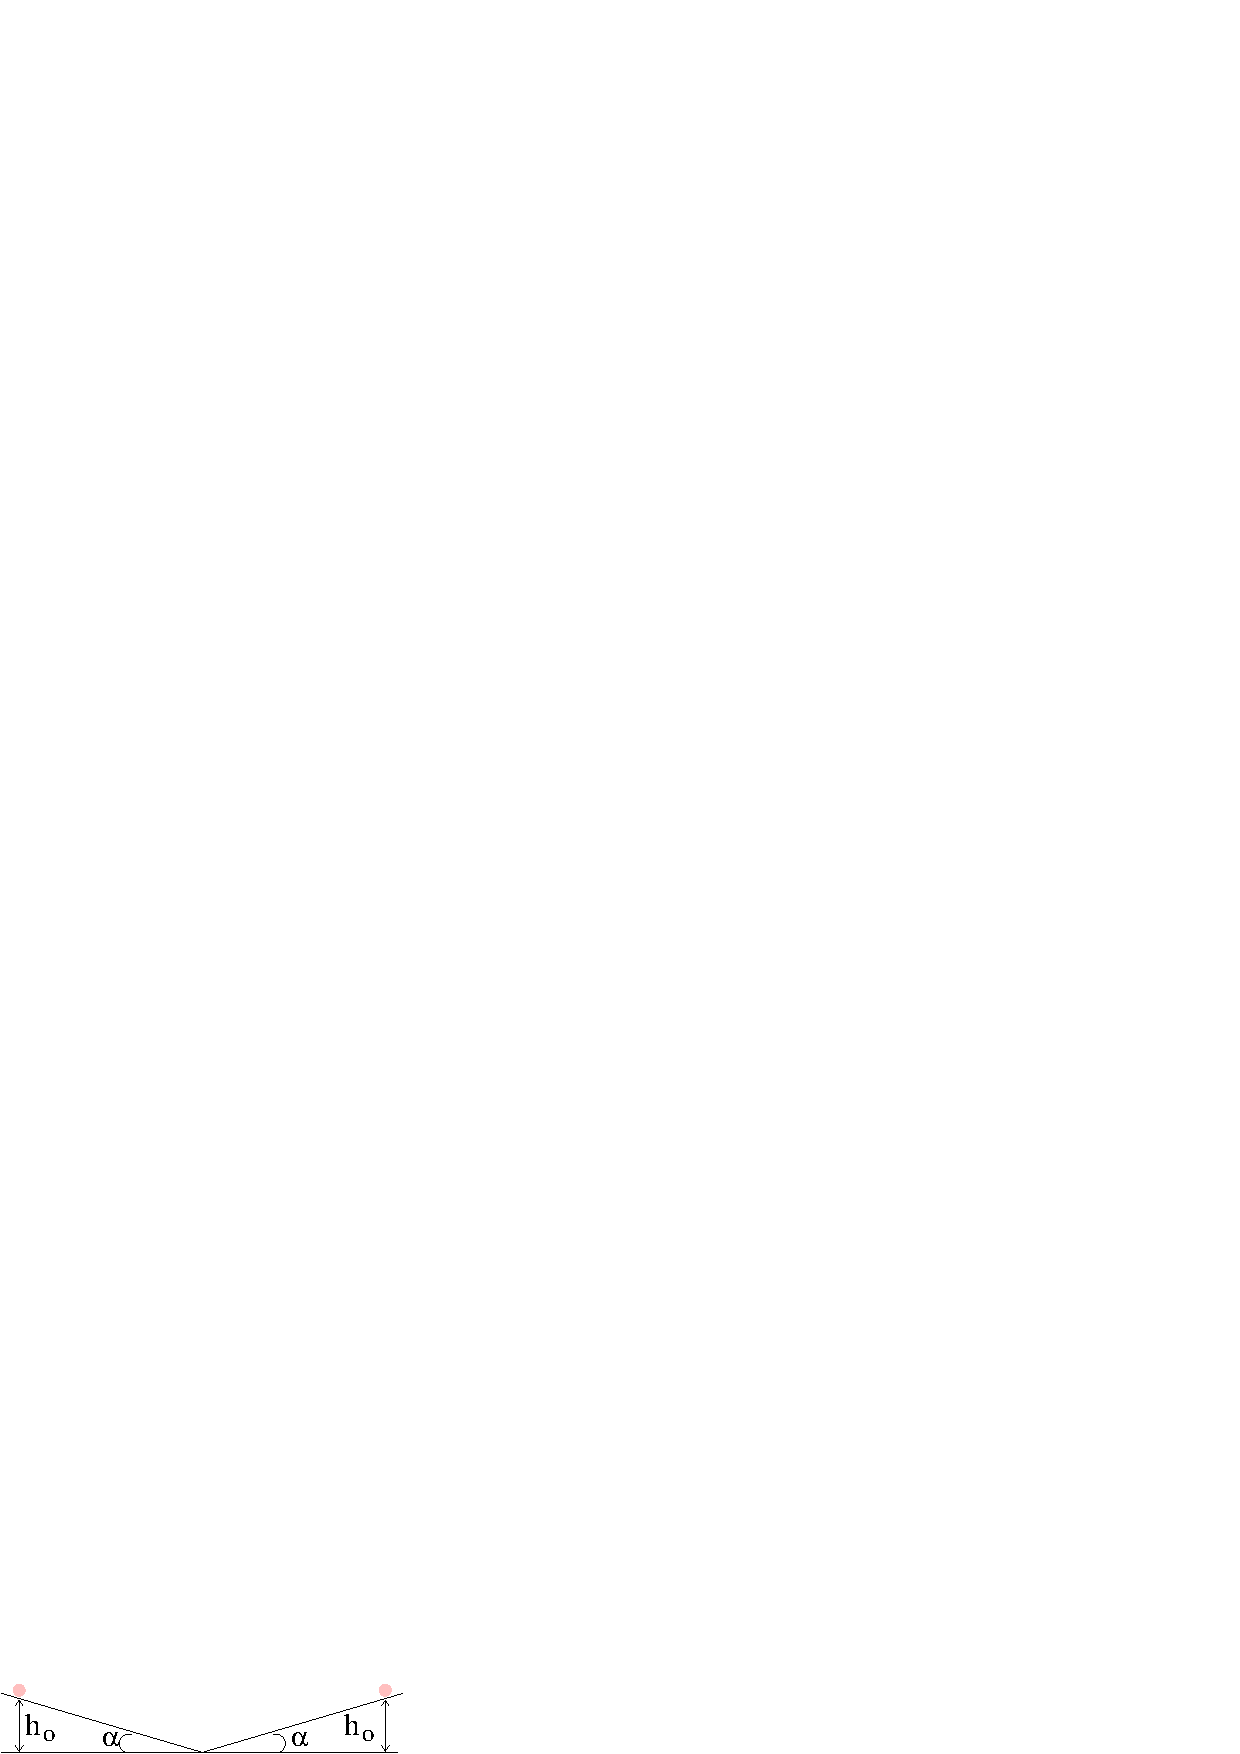
\includegraphics[width=\linewidth]{irudiak/08a-orria-biplano.png}
\end {minipage}
}
\begin{enumerate}
\item Encontrar el periodo del movimiento, si la altura inicial es $h_0$.
\item >Es un movimiento oscilatorio? >Es arm\'{o}nico simple?
\end{enumerate}

\item 
Supongamos que la elongaci\'{o}n en el equilibrio 
de un muelle al que se le ha suspendido
una masa  $m$  es  $l$. Demostrar  que si se perturba el sistema,
obtenemos el mismo movimiento que el de un p\'{e}ndulo simple de longitud
$l$.


\item 
\raisebox{-0.5cm}{
\begin{minipage}{0.7\linewidth}
Obtener la constante recuperadora del sistema formado por dos muelles de 
constantes  $k_1$ y $k_2$, cuando los muelles se colocan en serie
y cuando se colocan en paralelo (ver figura).
\end {minipage}
\hspace*{0.5cm}
\begin{minipage}{0.2\linewidth}
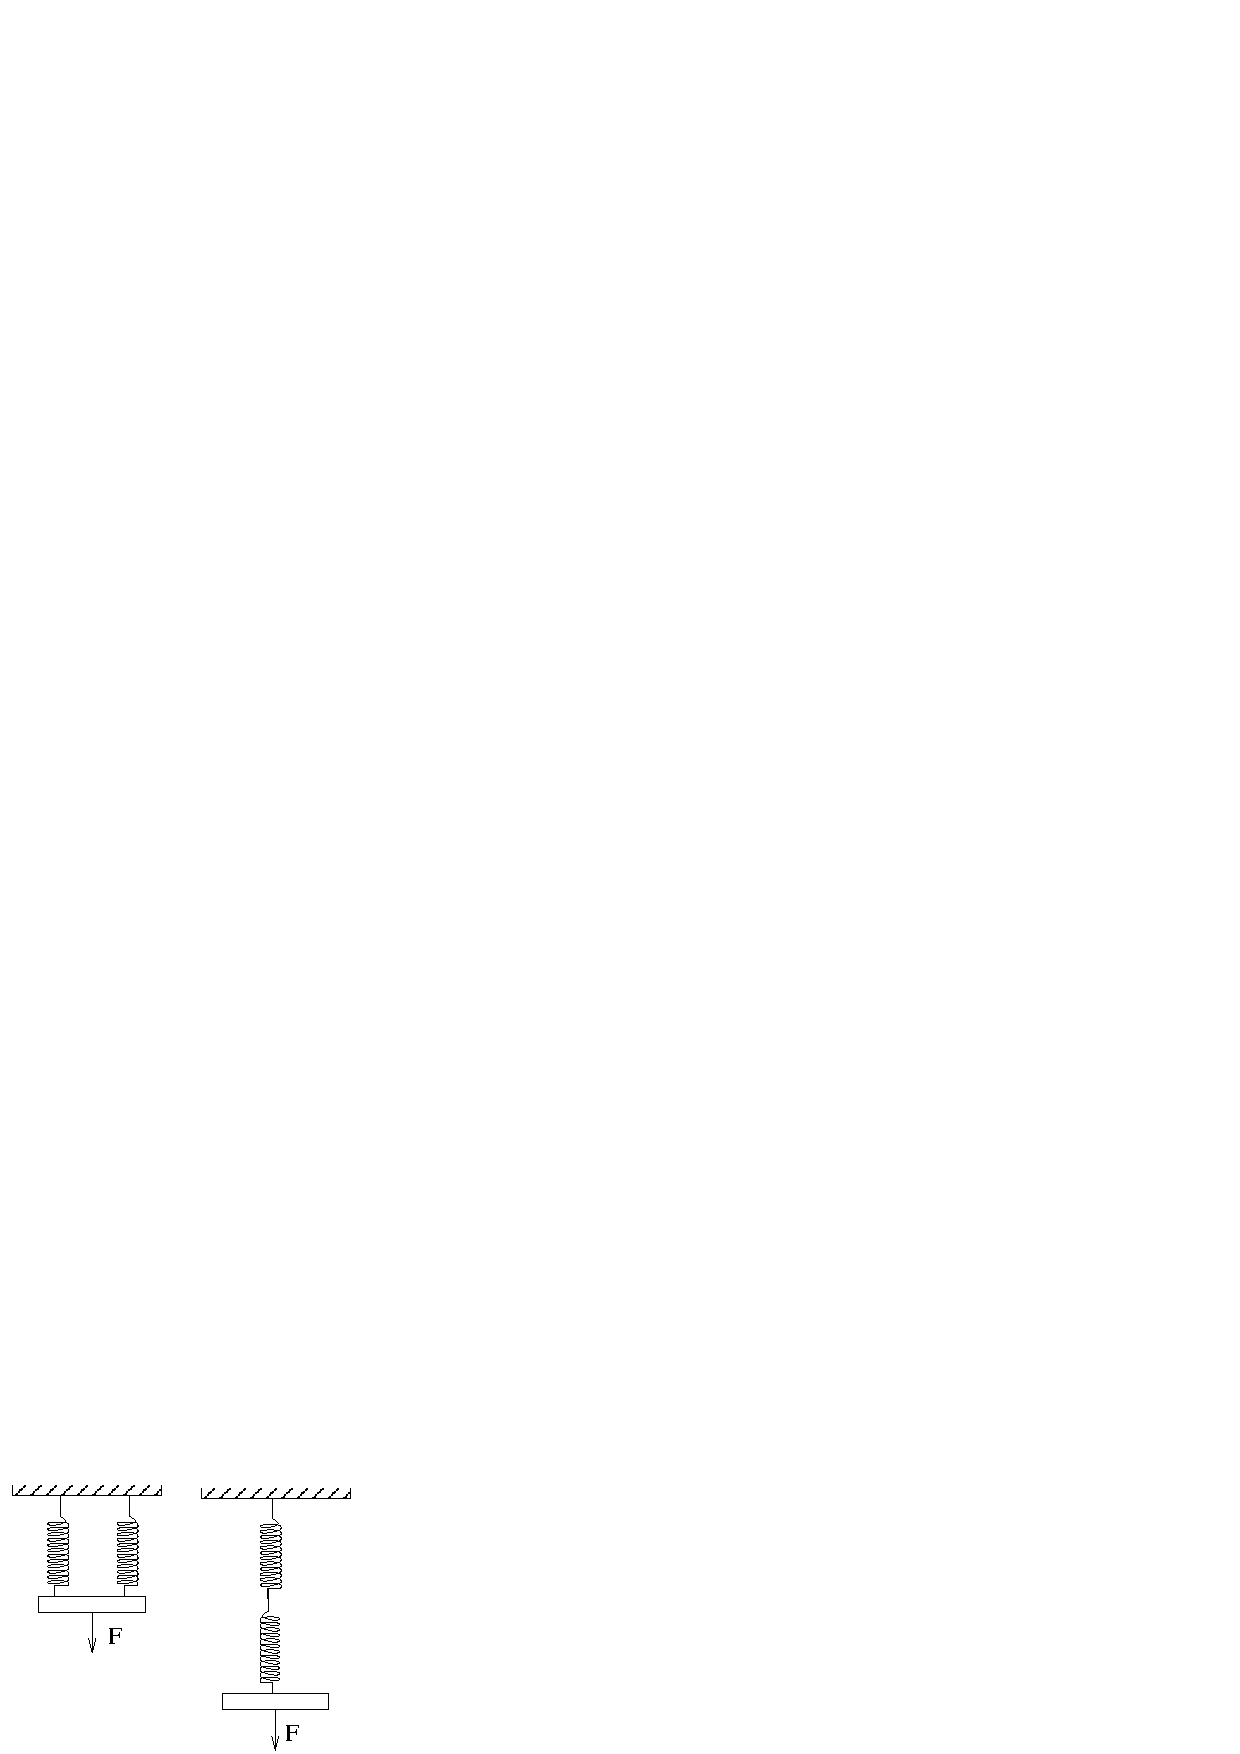
\includegraphics[width=\linewidth]{irudiak/08a-orria-malgukiser.png}
\end {minipage}
}


\item
Una masa de 2 kg  est\'{a} unida al extremo de un muelle.
La longitud propia del muelle es 8~cm, pero cuando la masa
se sit\'{u}a encima del muelle, la longitud del muelle es   5~cm.
Desde esta posici\'{o}n de equilibrio, se le da un golpe hacia
abajo y la part\'{\i}cula empieza a oscilar con una velocidad de 
0.3~m/s. 

\begin{enumerate}
\item >Cu\'{a}l es la altura m\'{a}xima que alcanza la masa?
\item >Cu\'{a}nto tiempo necesita la masa para alcanzar la 
altura m\'{a}xima por primera vez?
\item  >Estar\'{a} el muelle sin comprimir en alg\'{u}n instante? 
\item >Cu\'{a}l debe ser la velocidad inicial de la part\'{\i}cula para
que el  muelle est\'{e} sin comprimir en alg\'{u}n instante?
\end{enumerate}

\item
Una masa unida a un muelle horizontal oscila con un periodo de 4~s.
Si suspendemos la masa del mismo muelle, pero ahora en posici\'{o}n vertical
y sin oscilar, >cu\'{a}l es la elongaci\'{o}n del muelle?

\item
Una masa de 40 g realiza un movimiento arm\'{o}nico simple de periodo
T=0.32~s .
>Cu\'{a}l es la amplitud del movimiento si la fuerza m\'{a}xima 
que produce el movimiento vale 10 N?

\item
Un bloque de densidad relativa $\rho_r$  tiene forma de 
paralelep\'{\i}pedo de dimensiones  $a$, $b$ y $c$.
El bloque est\'{a} sobre agua, siendo el lado de longitud $a$
el vertical. Desde su posici\'{o}n de equilibrio, se le da un peque\~{n}o
golpe. Comprobar que el movimiento es arm\'{o}nico y
calcular la frecuencia angular de las oscilaciones. Ignorar el 
rozamiento. Ayuda: Escribir la segunda Ley de Newton para 
describir el movimiento del bloque.

\item
Cuando una masa de 2 kg se suspende de un muelle vertical lo alarga 10~cm.
Unimos la masa al mismo muelle y se pone sobre una mesa horizontal
y sin rozamiento, fijando el extremo del muelle que no tiene la masa a 
un punto fijo.
Separamos la masa 5~cm de su posici\'{o}n de equilibrio y la soltamos cuando
 t=0.
\begin {enumerate}
\item Obtener la amplitud, frecuencia angular, frecuencia y periodo.
\item Calcular la velocidad m\'{a}xima de la masa. >Cu\'{a}ndo ocurre?
\item Unimos una masa de 2~kg a un muelle de caracter\'{\i}sticas similares
pero se separa 10~cm de su posici\'{o}n de equilibrio. >Cu\'{a}l de las dos 
masas llegar\'{a} antes a su posici\'{o}n de equilibrio? >Por qu\'{e}? 
\item Separamos de nuevo la masa de su posici\'{o}n de equilibrio 
$3~$cm y se suelta con una velocidad inicial de $-25~$cm/s,
>cu\'{a}l  es la amplitud de las oscilaciones y la fase inicial?
\end{enumerate}

\item
Una masa $M$ est\'{a} sometida a 3 fuerzas:
La primera es perpendicular al eje $OY$ y vale $k_1\,x$.
La segunda es perpendicular al eje $OX$ y vale  $k_1\,y$.
La tercera est\'{a} dirigida a $O$y vale  $k_2\,r$, donde 
$r$ es la distancia al origen de coordenadas.
$k_1$ y $k_2$ son valores constantes.
Si la posici\'{o}n inicial de la masa es 
 (0,$a$) y su velocidad incial, $v_0$, es paralela al eje $OX$, encontrar:
\begin{minipage}{.49\linewidth}

\begin{center}
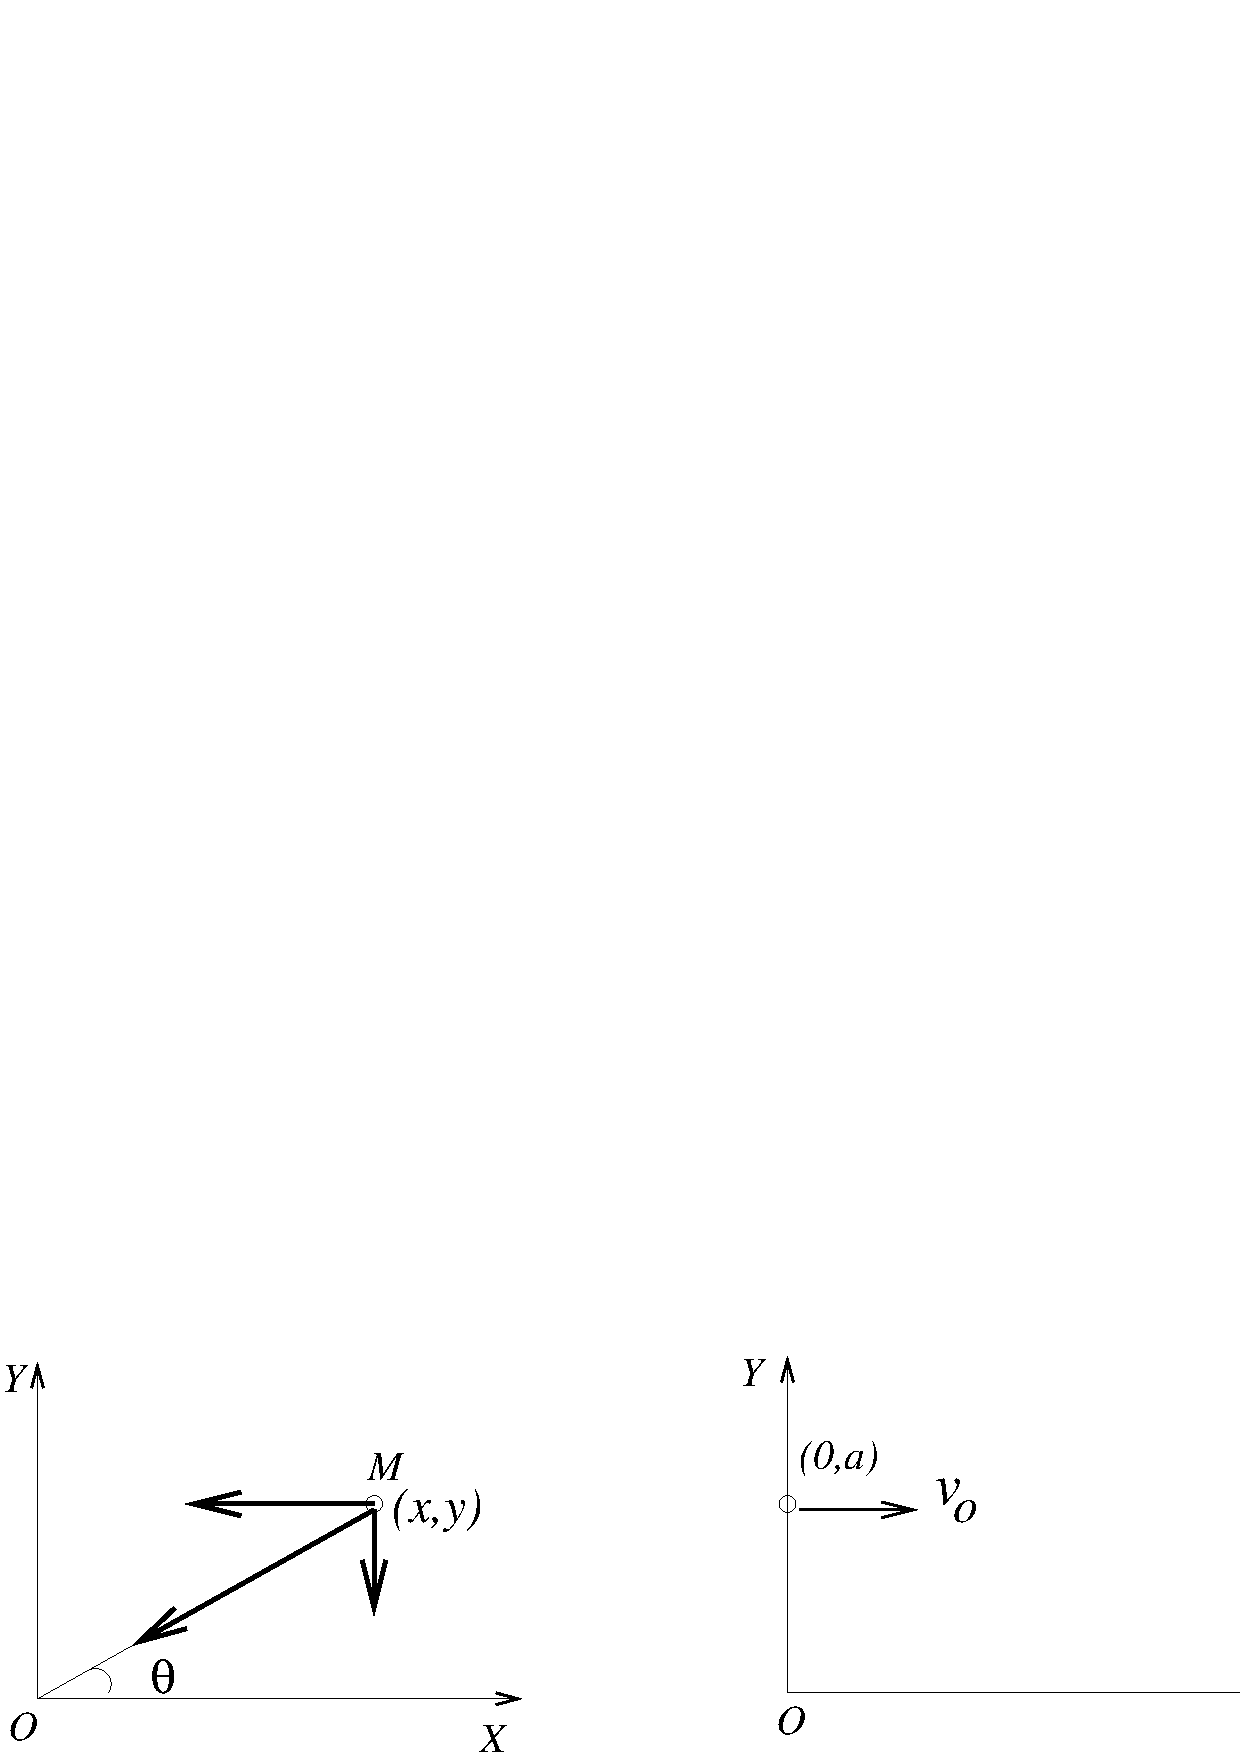
\includegraphics [width=\linewidth]{irudiak/3indar.png}
\end {center}
\end {minipage}\hfill
\begin{minipage}{.49\linewidth}
\begin{enumerate}
\item El tipo de movimiento y su periodo
\item Las ecuaciones param\'{e}tricas del movimiento
 (posici\'{o}n y velocidad en cualquier instante)
\item La ecuaci\'{o}n de la trayectoria. >Qu\'{e} tipo de curva es?
\end{enumerate}
\end {minipage}


\item 
\raisebox{-0.3cm}{
\begin{minipage}{0.80\linewidth}
El anillo de la figura de masa  $m$ y radio
$R$, se suspende del punto  $O$ y realiza peque\~{n}as oscilaciones en el plano vertical. >Cu\'{a}l es el periodo de las oscilaciones?
\end {minipage}
\hspace*{0.5cm}
\begin{minipage}{0.15\linewidth}
\includegraphics [width=0.8\linewidth]{irudiak/08a-orria-pendufisikoa.png}
\end {minipage}
}


\item
\raisebox{-0.8cm}{
\begin{minipage}{0.10\linewidth}
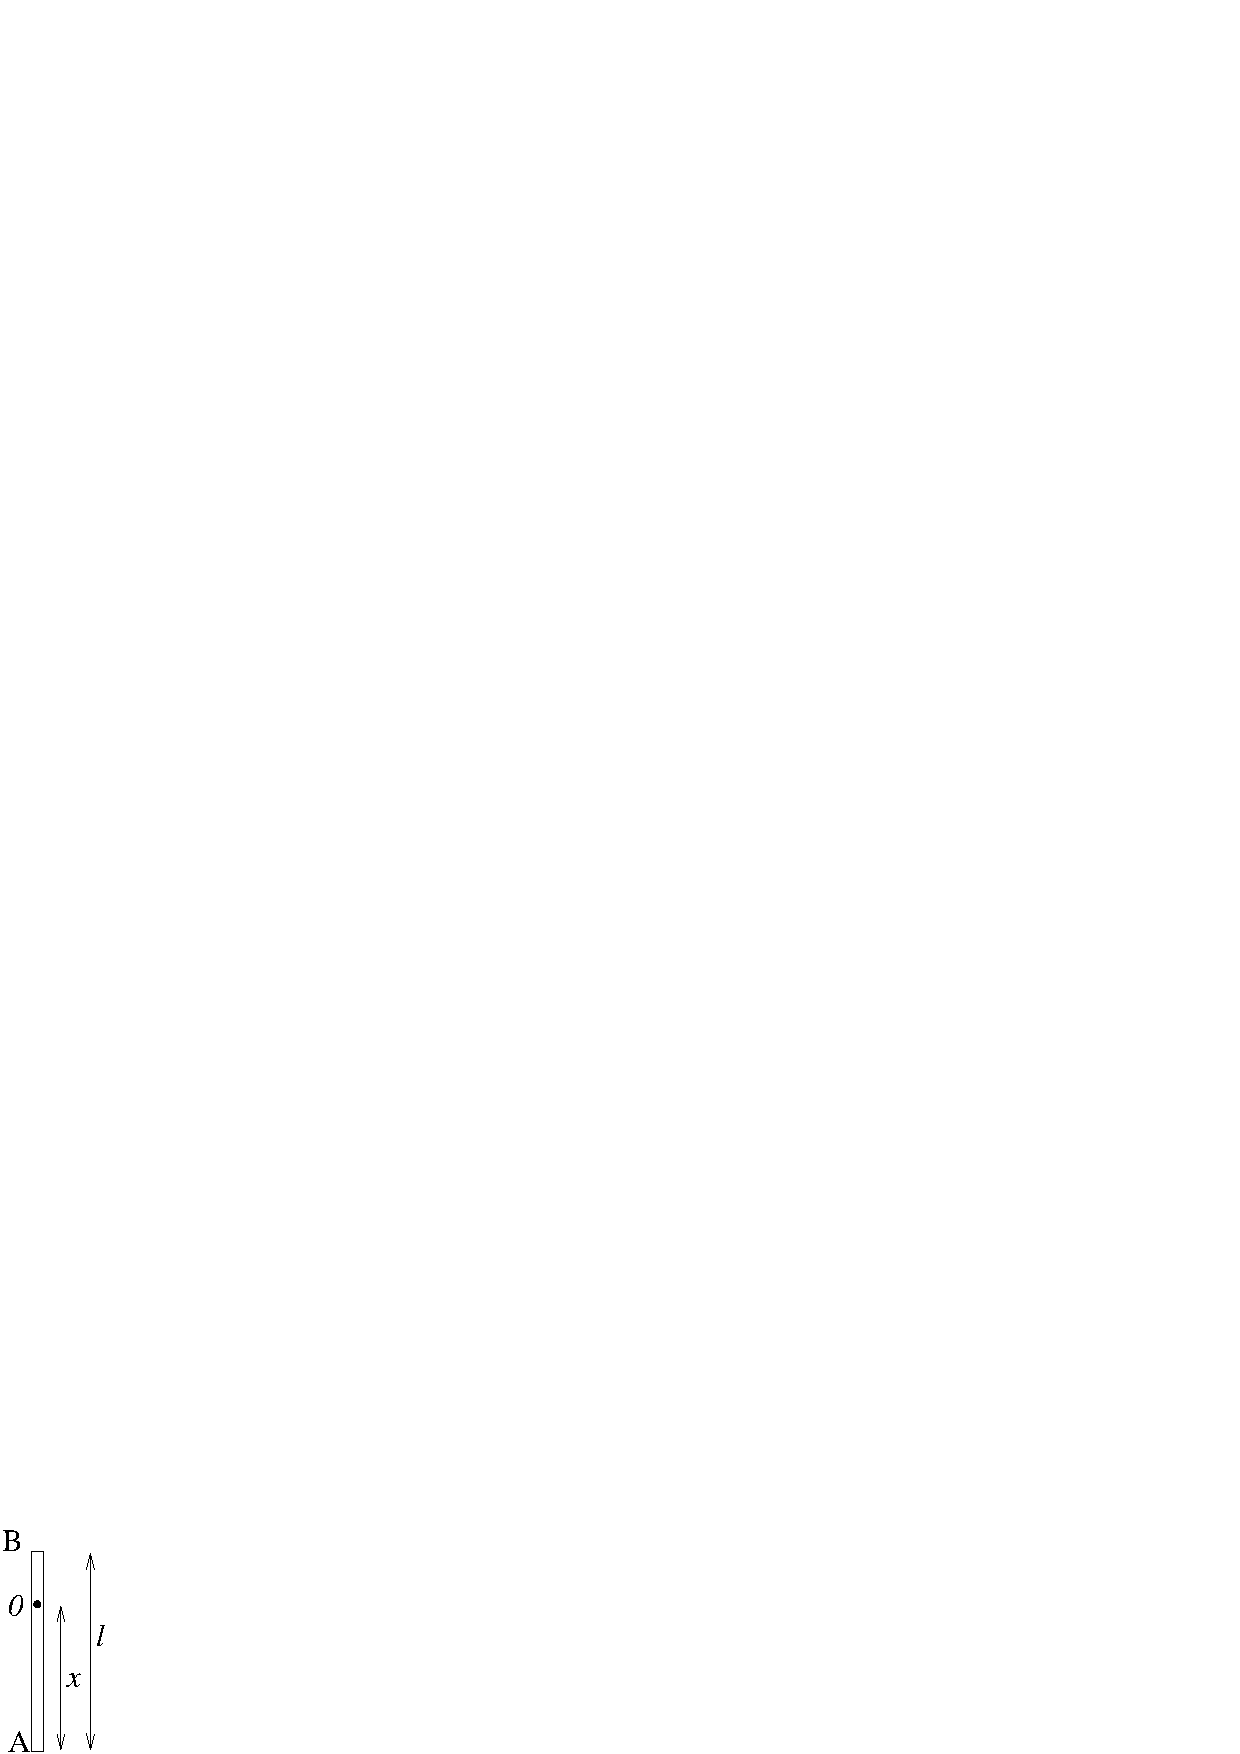
\includegraphics [width=\linewidth]{irudiak/08a-orria-makila.png}
\end {minipage}
\hspace*{0.5cm}
\begin{minipage}{0.80\linewidth}
Una barra pesada est\'{a} suspendida del punto $O$ y realiza peque\~{n}as
oscilaciones
en la vertical  alrededor de un eje perpendicular que pasa por $O$.
 >Cu\'{a}l debe ser la distancia  $x$  indicada
en el dibujo, para que el periodo de las oscilaciones sea m\'{\i}nimo?
\end {minipage}
}


\item
\raisebox{-1.3cm}{
\begin{minipage}{0.80\linewidth}
Un objeto plano tiene momento de inercia  $I$  respecto del 
eje perpendicular que pasa por su centro de masas.
Cuando oscila alrededor del punto  $P_1$ (ver figura) su periodo es  $T$.
Al otro lado del centro de masas, puede encontrarse otro punto,  $P_2$,
respecto del cual el periodo de oscilaci\'{o}n tambi\'{e}n es  $T$.
Demostrar que la distancia entre los puntos  $P_1$ y $P_2$ es
$gT^2/(4\pi^2)$.
\end {minipage}
\hspace*{0.5cm}
\begin{minipage}{0.15\linewidth}
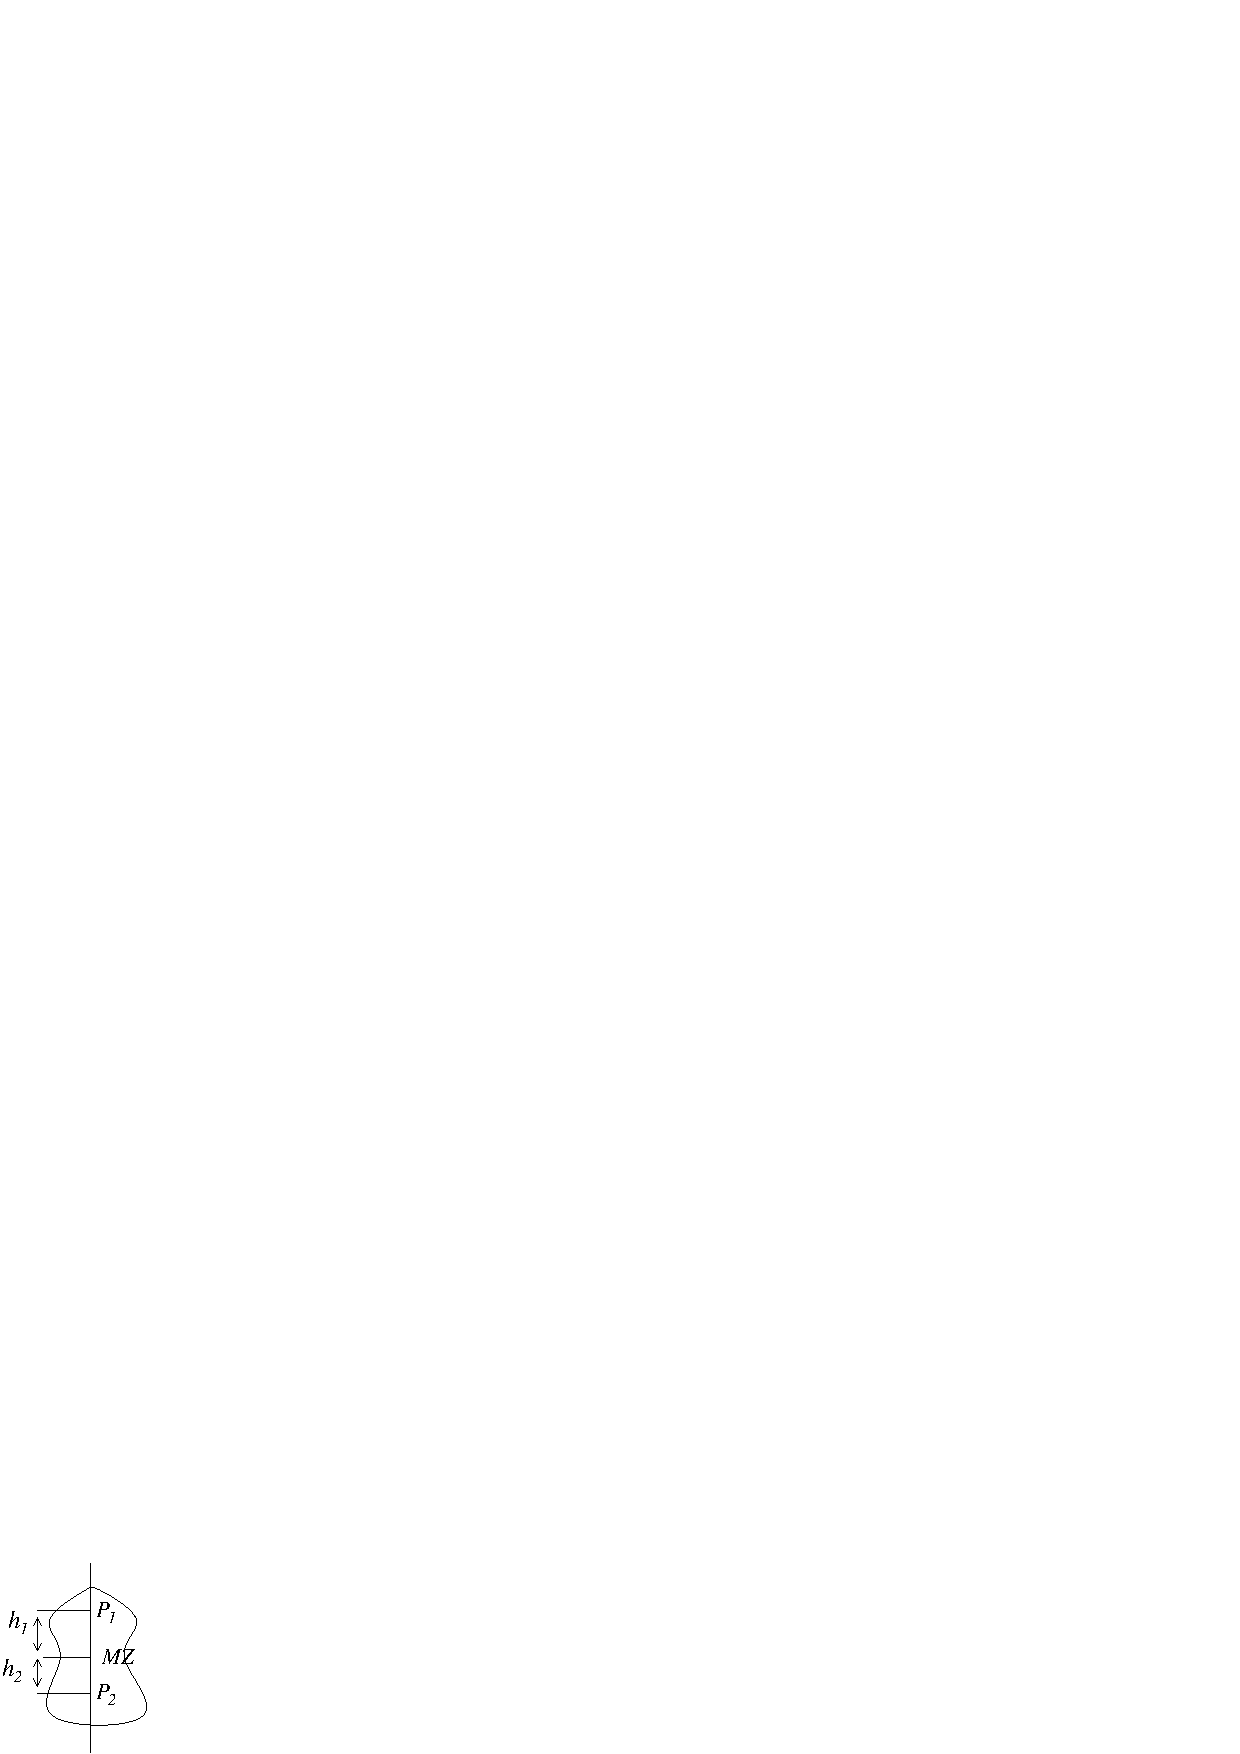
\includegraphics [width=\linewidth]{irudiak/08a-orria-P1P2.png}
\end {minipage}
}

\newpage
\item
El periodo de un p\'{e}ndulo simple vale $2.5\,{\rm s}$ cuando realiza
peque\~{n}as oscilaciones. En un momento dado la amplitud del movimiento 
vale $2^{\rm o}$.  A causa del rozamiento,  la amplitud
va disminuyendo hasta que al cabo de 10 oscilaciones la amplitud vale
 $1.5^{\rm o}$. Obtener el factor de amortiguamiento.

\item
El tiempo de relajaci\'{o}n de una oscilador amortiguado se define como:
 $\tau=1/(2\gamma)$, donde $\gamma$ es el factor de amortiguamiento.
>Cuáles son las unidades del tiempo de relajaci\'{o}n? >Cu\'{a}l es el 
cambio en la amplitud del oscilador  al cabo de un tiempo $\tau$?


\end{enumerate}

{\bf Resultados }

%\begin{multicols}{2}{
\begin{enumerate}
\item[1.] $a$) x$\le0,031$~m; $b$) $\nu_{max}$=3,16~s$^{-1}$
\item[2.] $T=\frac{4}{\sin\alpha}\sqrt{\frac{2h_o}{g}}$
%\item[3.] $\bar{x}$=0; $\bar{x^2}=\frac{1}{2}A^2$
\item[4.] $K_{par}=k_1+k_2$; $\frac{1}{K_{ser}}=\frac{1}{k_1}+\frac{1}{k_2}$
\item[5.] a)$h_{max}=$17~mm, b)0.26~s, d)0,54~m/s
\item[6.] $x$= 3,97~m
\item[7.] A=65~cm
\item[8.]  $\omega=\sqrt{g/(\rho_r a)}$
\item[9.] a)$A$=5~cm, $f$=1.58~Hz, $T=0,6347$~s b) $v_{max}$=0.495~m/s, t=0.158~s
   d) $\varphi$= 2.26~rad, $A$=3.91~cm
\item[11.] $T=2\pi\sqrt{\frac{2R}{g}}$; ($I=2MR^2$)
\item[12.] $x=l\frac{3+\sqrt{3}}{6}$; ($I=\frac{1}{12}ml^2+m(x-l/2)^2))$
\item[14.] $\gamma$=0,0115 s$^{-1}$
\item[15.] 0,606

\end{enumerate}
%}\end{multicols}


\end {document}
